%%%%%%%%%%%%%%%%%%%%%%%%%%%%%%%%%%%%%%%%%
%
% Space Physics
% Practical 2B
%
%%%%%%%%%%%%%%%%%%%%%%%%%%%%%%%%%%%%%%%%%

%----------------------------------------------------------------------------------------
%	DOCUMENT CONFIGURATIONS
%----------------------------------------------------------------------------------------

\documentclass{article}

\title{\textbf {Space Physics} \\ Practical 2B\\ Data Analysis} % Title
\def\authorivan{Ivan \v Sinkarenko}
\def\authoranu{Anuraj Rajendraprakash}
\author{\authorivan\\\authoranu}

\usepackage{graphicx}
\usepackage{fullpage}
\usepackage{url}
%\usepackage{color}

% load package with ``framed'' and ``numbered'' option.
\usepackage[framed,numbered,autolinebreaks,useliterate]{mcode}

\begin{document}

\maketitle % Insert the title, author and date

\centerline{Referee: Gabriella Stenberg}

\setlength\parindent{0pt} % Removes all indentation from paragraphs

\renewcommand{\labelenumi}{\alph{enumi}} % Make numbering in the enumerate environment by letter rather than number
\clearpage

\tableofcontents

\listoffigures

\clearpage

%----------------------------------------------------------------------------------------
%	SECTION 1. Introduction
%----------------------------------------------------------------------------------------
\section{Introduction}

    

%----------------------------------------------------------------------------------------
%	SECTION 2. Time Series Data
%----------------------------------------------------------------------------------------
\section{Time Series Data}

\subsection{Question 1}
The measurment taken on 2002-03-02 at 03:29-03:30 is taken at the time when the satellite was crossing the border of magnetopause.

\begin{figure}[htb]
\centering
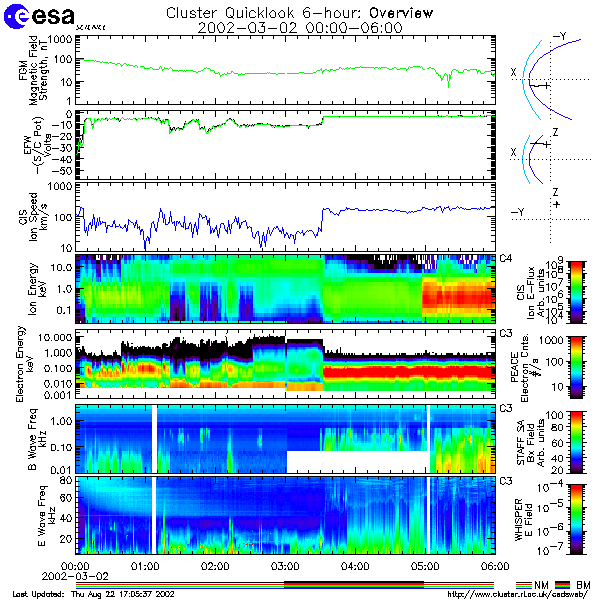
\includegraphics[width=0.7\textwidth]{Figures/cluster.png}
\caption{Cluster Quicklook 6-hours overview.}
\label{fig:cluster}
\end{figure}

\subsection{Question 2}

Electromagnetic between 20 and 30 s. Electrostatic between 55 and 60 s. x component is facing towards the sun. It should fluctuate around zero, like the y-component does it. It happens because of the photon emission, which is captured by the probes. Thus, data correction is needed.

\begin{figure}[htb]
\centering
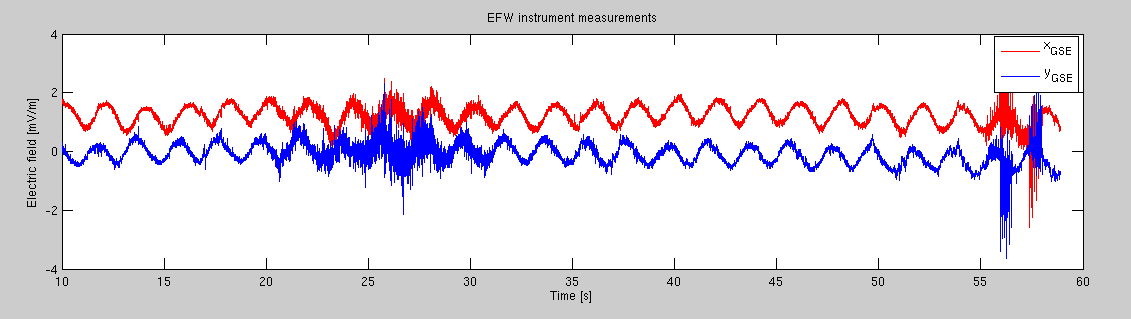
\includegraphics[width=\textwidth]{Figures/EFW_measurement.png}
\caption{EFW Measurement Data}
\label{fig:EFW}
\end{figure}

\begin{figure}[htb]
\centering
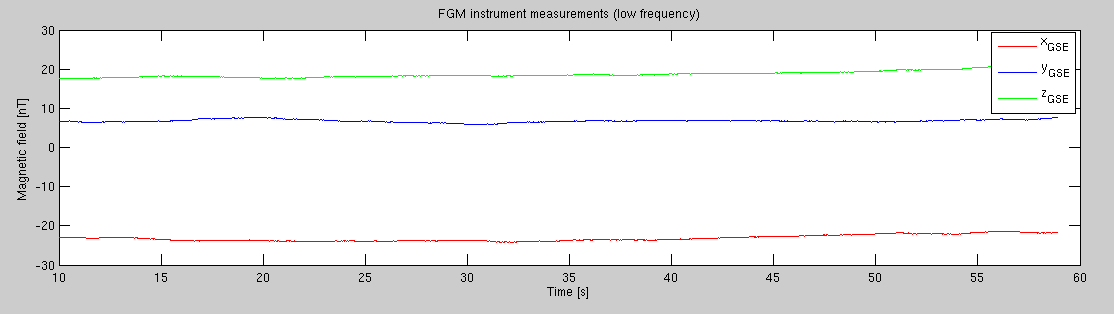
\includegraphics[width=\textwidth]{Figures/FGM_measurement.png}
\caption{FGM Measurement Data}
\label{fig:FGM}
\end{figure}

\begin{figure}[htb!]
\centering
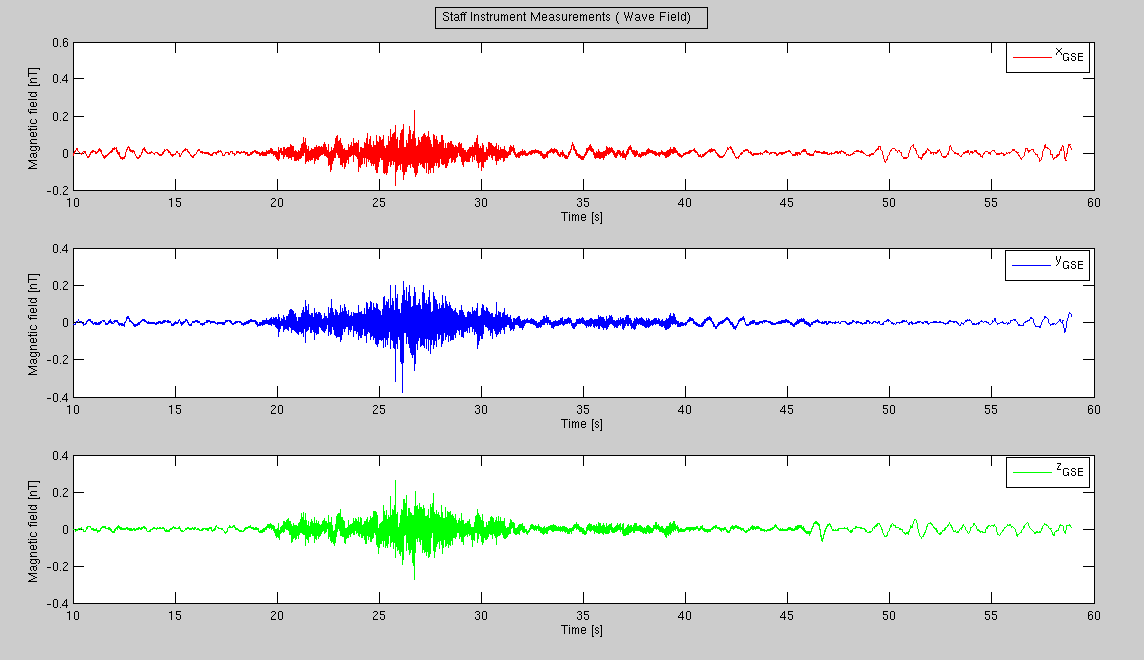
\includegraphics[width=\textwidth]{Figures/Staff_measurement.png}
\caption{Staff Instrument Measurement Data}
\label{fig:Staff}
\end{figure}

\subsection{Question 3}
Roughly estimated wave period is about 0.01 s (zoomed in and estimated between 2 peaks). Frequency = 1/0.01 = 100 Hz.

\subsection{Question 4}
From overview data, ion density is $~1.5 cm^3$. 

The estimated plasma frequency from WHISPER is 16 kHz.

\subsection{Question 5}
The peaks are around 90-100 Hz. Which corresponds to our rough estimation in question 3.

\clearpage
%----------------------------------------------------------------------------------------
%	SECTION 2. PARTICLE MEASUREMENTS
%----------------------------------------------------------------------------------------
\section{Particle Measurements}

For this part of the practical we have been provided the particle data from the SWIM
instrument onboard the Chandrayaan-1 spacecraft. Chandrayaan-1 orbits the moon at an altitude of 100 km. The position of the spacecraft at different times is shown in the Figures \ref{fig:orbit_1069} and \ref{fig:orbit_1070}, which also show the position of the moon with respect to Earth.

\begin{figure}[ht]
\begin{minipage}[c]{0.5\linewidth}
\centering
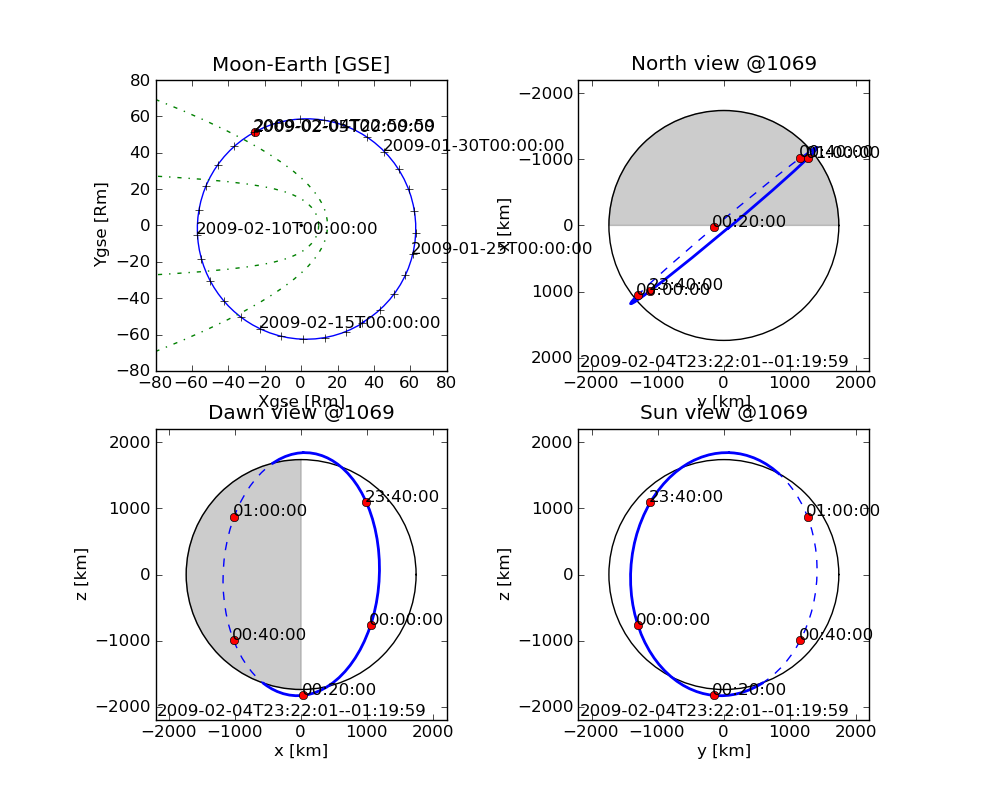
\includegraphics[width=9cm]{Figures/orbit_1069.png}
\caption{Position of the instrument in Orbit 1069}
\label{fig:orbit_1069}
\end{minipage}
\hspace{0.2cm}
\begin{minipage}[c]{0.5\linewidth}
\centering
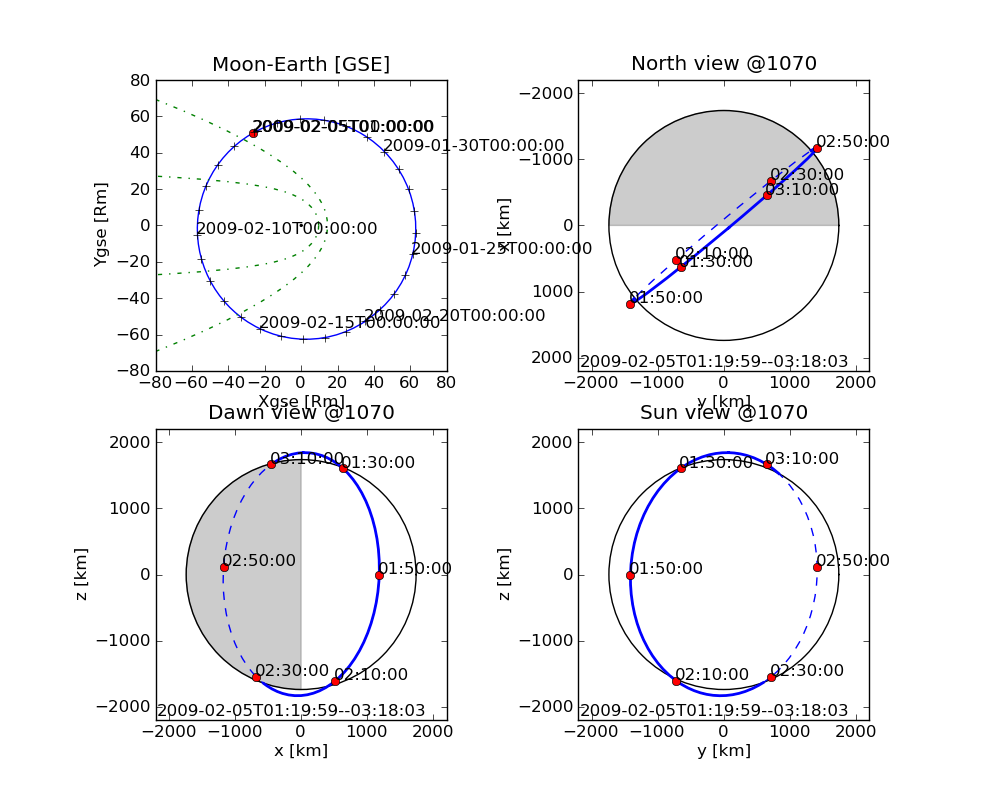
\includegraphics[width=9cm]{Figures/orbit_1070.png}
\caption{Position of the instrument in Orbit 1070}
\label{fig:orbit_1070}
\end{minipage}
\end{figure}


\subsection{Question 1}
\textit{Plot spectrograms, that is, the number of counts versus time and energy, for the
two orbits. The different energy levels you find in a comment line in the data files.
Once every orbit SWIM looks at the solar wind. Identify when this happens in the two
orbits.}

The spectrograms for the orbits 1069 and 1070 is shown in Figure \ref{fig:spectrogram_1069} and \ref{fig:spectrogram_1070} respectively. When SWIM looks at the solar wind the number of solar wind particles that hit the instrument increases significantly which is observable as the red portion in Figures \ref{fig:spectrogram_1069} and \ref{fig:spectrogram_1070}. For orbit 1069, it occurs approximately between $100th$ and $350th$ observation time bin which corresponds to UTC 05:29 to UTC 06:02 hours. For orbit 1070, it occurs approximately between $25th$ and $250th$ observation time bin which corresponds to UTC 07:22 to UTC 08:12 hours.

\begin{figure}[h!]
\centering
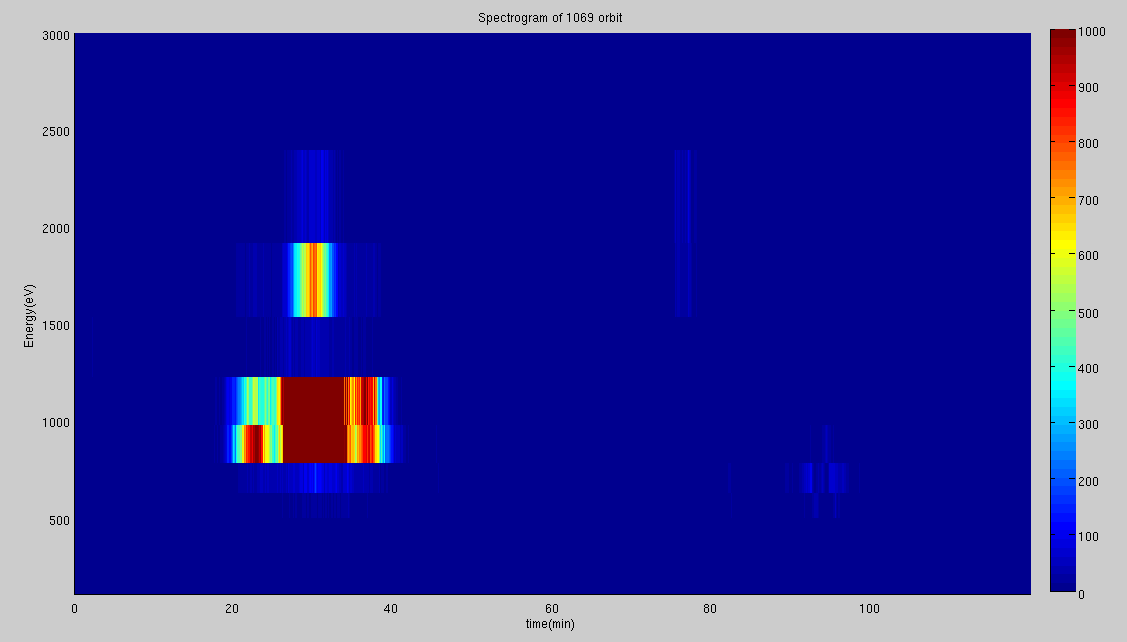
\includegraphics[scale=0.35]{Figures/spectrogram_1069.png}
\caption{Spectrogram of the 1069 Orbit}
\label{fig:spectrogram_1069}
\end{figure}

\begin{figure}[h!]
\centering
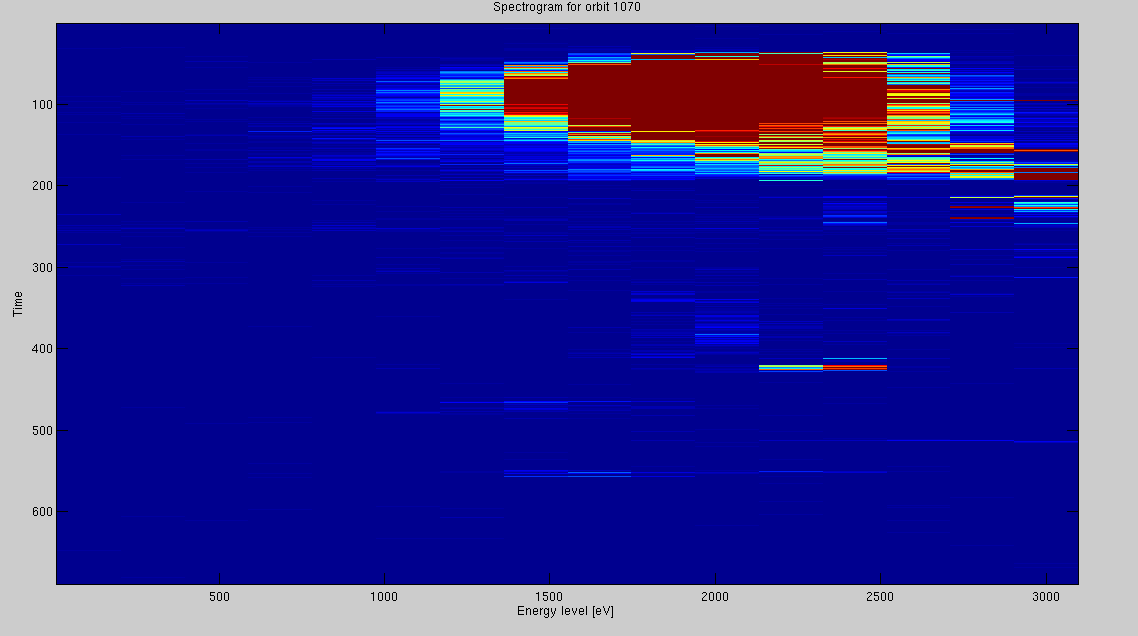
\includegraphics[scale=0.35]{Figures/spectrogram_1070.png}
\caption{Spectrogram of the 1070 Orbit}
\label{fig:spectrogram_1070}
\end{figure}

\subsection{Question 2}
\textit{Protons are the main ions in the solar wind, but can you identify any other
components? Motivate you answer!}

{\color{red} Helium double plus. I am not sure.}

\subsection{Question 3}
\textit{Make energy spectra, this is, plot observed counts versus energy for a selected
time interval around the solar wind observation.}

The energy spectra for the time when the SWIM instrument looks at the solar wind for the orbit 1069 and orbit 1070 is shown in Figure \ref{fig:energy_spectra_1069} and \ref{fig:energy_spectra_1070} respectively

\begin{figure}[h!]
\centering
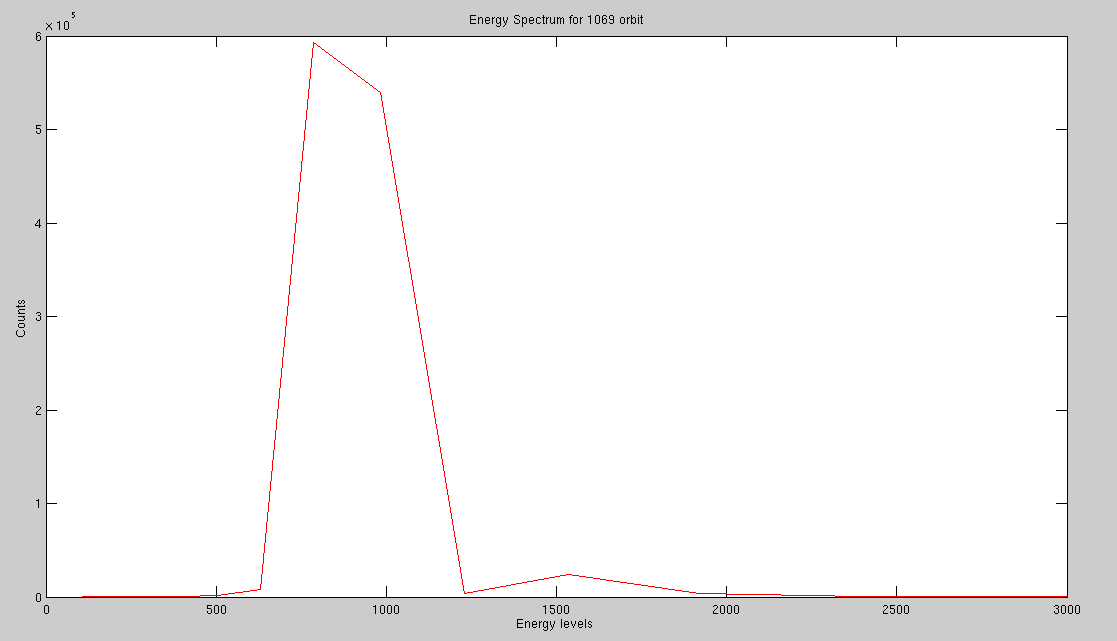
\includegraphics[scale = 0.35]{Figures/energy_spectra_1069.png}
\caption{Energy Spectra of the 1069 Orbit}
\label{fig:energy_spectra_1069}
\end{figure}

\begin{figure}[h!]
\centering
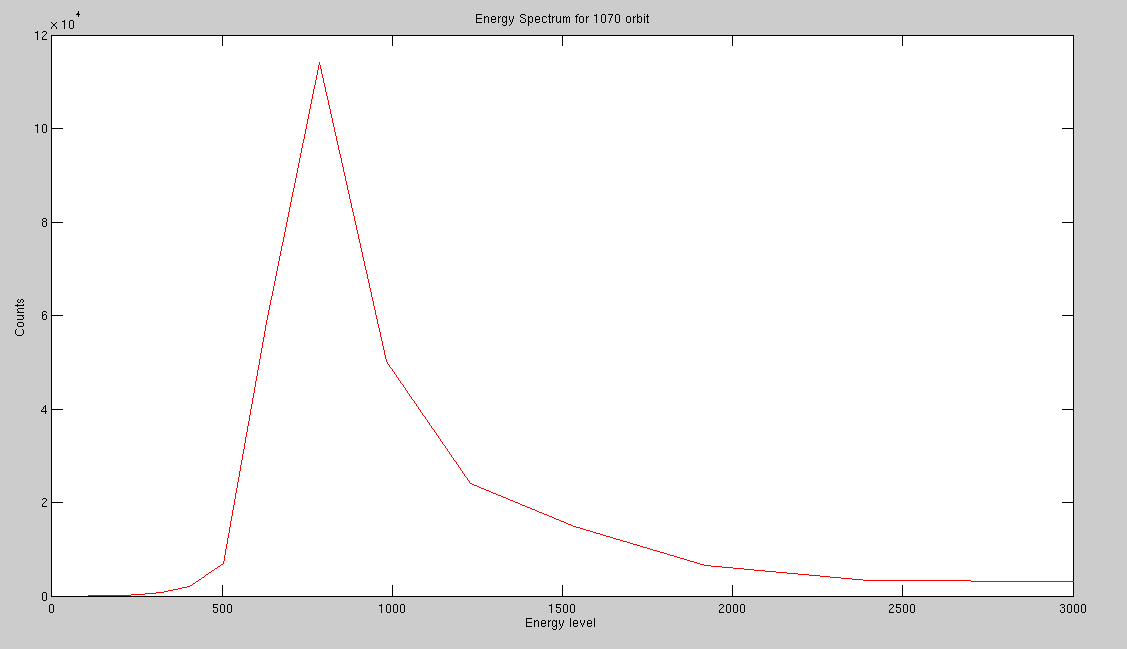
\includegraphics[scale = 0.35]{Figures/energy_spectra_1070.png}
\caption{Energy Spectra of the 1070 Orbit}
\label{fig:energy_spectra_1070}
\end{figure}

\subsection{Question 4}
\textit{Determine the solar wind proton velocity and temperature by first transforming the
data from energy to velocity space and then fitting a Maxwellian distribution. What
temperatures and velocities do you get? Are there differences between the orbits? If
so, why?}

\begin{figure}[!ht]
\centering
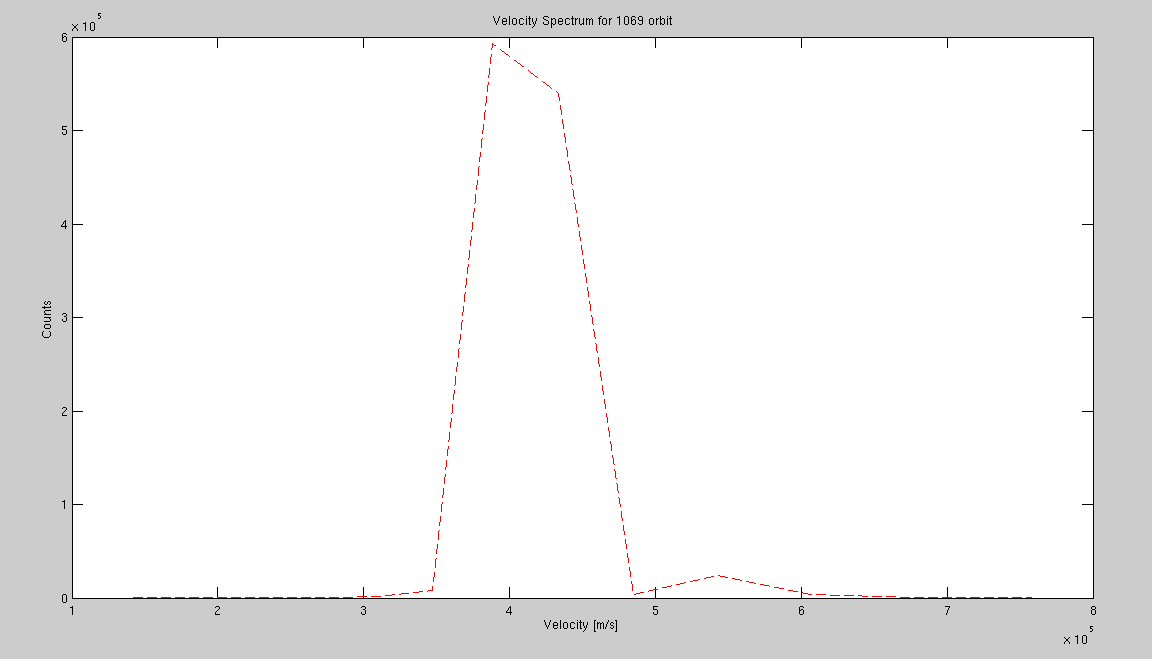
\includegraphics[scale=0.35]{Figures/velocity_spectra_1069.png}
\caption{Velocity Spectra of the 1069 Orbit}
\label{fig:Velocity_spectra_1069}
\end{figure}

\begin{figure}
\centering
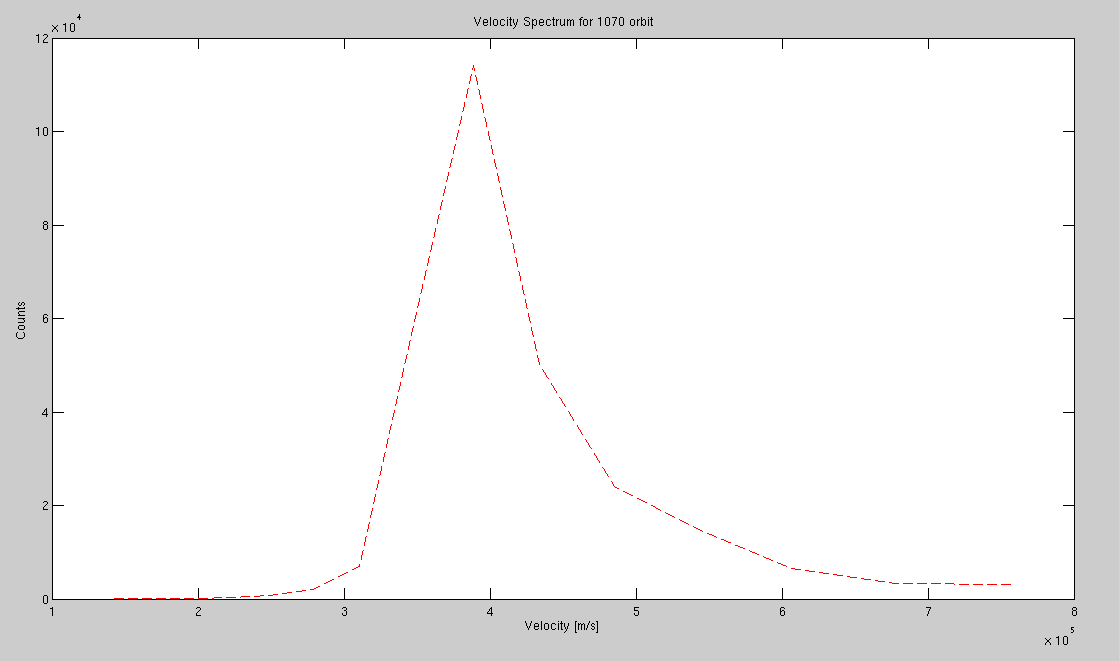
\includegraphics[scale=0.35]{Figures/velocity_spectra_1070.png}
\caption{Velocity Spectra of the 1070 Orbit}
\label{fig:Velocity_spectra_1070}
\end{figure}

\begin{figure}[!ht]
\centering
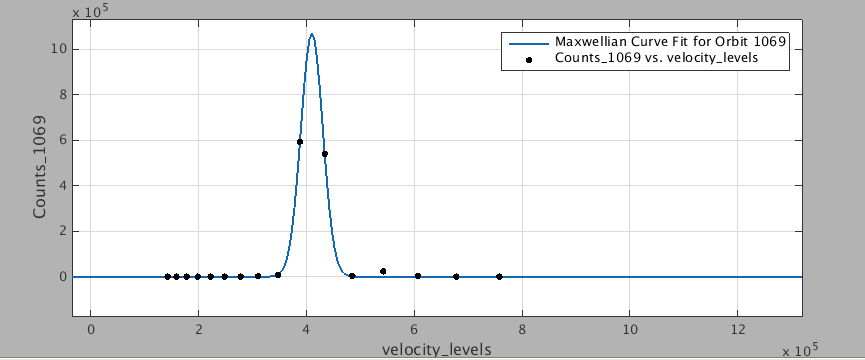
\includegraphics[scale=0.45]{Figures/curvefit_1069.png}
\caption{Maxwellian Curve fit for data from Orbit 1069}
\label{fig:curvefit_1069}
\end{figure}

\begin{figure}
\centering
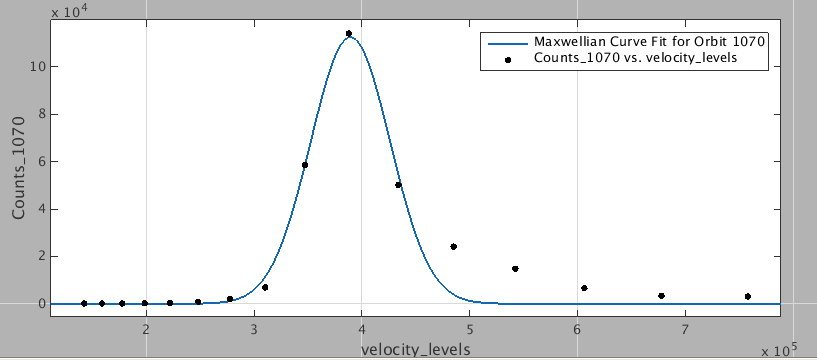
\includegraphics[scale= 0.45]{Figures/curvefit_1070.png}
\caption{Maxwellian Curve fit for data from Orbit 1070}
\label{fig:curvefit_1070}
\end{figure}


%----------------------------------------------------------------------------------------
%	SECTION 3. CONCLUSION
%----------------------------------------------------------------------------------------
%\newpage
\section{Conclusion}



%----------------------------------------------------------------------------------------
%	SECTION 4. REFERENCES
%----------------------------------------------------------------------------------------
\newpage
\begin{thebibliography}{9}

\bibitem{Enmark:2012a3}
Enmark A.  (2012).
\newblock {\em Assignment 3. Optimization of phased array antenna radiation pattern and array configuration}.
\newblock Lule\aa \ University of Technology, Kiruna, Sweden.

\bibitem{Skolnik:2001irs}
Skolnik M. ~I.  (2001).
\newblock {\em Introduction to Radar Systems}.
\newblock The McGraw-Hill Companies, Inc., New York, United States.

\bibitem{Rottger:2000ip}
R\"ottger J.  (2000).
\newblock {\em The Instrumental Principles of MST Radars and Incoherent Scatter Radars and The Configuration of Radar System Hardware}.
\newblock Max Planck Institut F\"ur Aeronomie, Katlenburg-Lindau, Germany.

\bibitem{Wiki:2012pa}
Wikipedia.org. (2012).
\newblock {\em Phased array}.
\newblock {\url{http://en.wikipedia.org/wiki/Phased_array}}.

\end{thebibliography}


%----------------------------------------------------------------------------------------
%	SECTION 5. Appendix 1
%----------------------------------------------------------------------------------------
\newpage
\section{Appendix 1. Matlab code}
%\lstinputlisting{assignment.m}

\end{document}